\chapter{Analyzing Optimizer Behavior}

This chapter provides a brief overview of some of the tools provided in Mesquite for assisting with the analyze and visualization of the Mesquite optimization process.  The tools discussed in this section can be used to provide additional
output.  External tools such as Paraview, VisIt, or GNU Plot must be used to visualize the data.

\section{Debug Output}

Mesquite contains a mechanism to send status and debug messages to an output stream (e.g. {\texttt stdout} or {\texttt std::cout}).  Debug messages are grouped into logical categories identified by an integer number.  For example debug flag 1 refers to warnings.  Debug flag 2 is used for status information about the outer optimization loop, and debug flag 3 is used for status of the inner optimization loop. 

Debug flags can be controlled through a variety of means.  The {\texttt --enable-debug-output} configure option can be specified with a comma-separated list of integer values to specify which debug groups should be enabled by default.  An application may call the {\texttt MsqDebug::enable(unsigned)} and {\texttt MsqDebug::disable(unsigned)} functions to enable or disable debug message groups.  Debug message groups may also be controlled with the environmental variables {\texttt MESQUITE\_DEBUG} and {\texttt MESQUITE\_NO\_DEBUG}.  Each should have a comma-separated list of integer values as its argument.  The variables enable and disable, respectively, the corresponding debug message groups.

\section{Plotting Convergence Behavior \label{sec:optplot}}

The Mesquite {\texttt TerminationCriterion} class can produce a simple table of tab-separated values for the different Mesquite termination criterion.  This file can be used to plot the behavior of the optimization loop using GNU Plot, a spread sheet application, or any other suitable tool.  The code listing below illustrates how this feature is activated.

\begin{lstlisting}[frame=single]
// Create global optimizer instance
SteepestDescent improver( &objective_function );
improver.use_global_patch();

// Set only inner termination criterion for 
// global optimization
TerminationCriterion inner;
inner.add_absolute_vertex_movement( 1e-3 );
\<inner.write_iterations( "plot.gpt" );\>
improver.set_inner_termination_criterion( &inner );

// Run optimization
InstructionQueue queue;
queue.set_master_quality_improver( &improver, err );
queue.run_instructions( &mesh, err );
\end{lstlisting}

For usable results the feature must be activated on the appropriate {\texttt TerminationCriterion} instance.  For a global optimization it should be enabled for the {\em inner} termination criterion.  For other optimization strategies (see Chapter \ref{ch:optstrat}) it should be enabled for the {\em outer} termination criterion.  

The following is a sample output file:

\begin{lstlisting}[basicstyle=\small,language=sh]
#Iter	CPU	ObjFunc	GradL2	GradInf	Movement	Inverted
0	0	1.47419	0	0	0	0
1	0	1.147	0	0	0.657155	0
2	0	1.04779	0	0	0.402173	0
3	0	1.00572	0	0	0.357444	0
4	0	1.00006	0	0	0.150652	0
5	0	1	0	0	0.0153396	0
6	0	1	0	0	0.00015034	0
7	0	1	0	0	6.40008e-09	0
\end{lstlisting}

Notice that several of the columns contain only zeros.  The column containing the iteration number will always contain valid values.  Other values will only be included if they are calculated during the optimization loop.  The objective function value will be included for any global optimization that uses an explicit objective function (currently any optimizer other than {\texttt LaplacianSmoother}).  In the example source code above we are using the steepest descent solver with a global patch so the objective function value is also included.  The other values will only be present if they are calculated for the purpose of checking termination criteria.  In the example source code we specify a termination criterion based on vertex movement, so the column labeled ``movement'' contains the maximum distance any vertex was moved for the corresponding iteration.  

Figures \ref{fig:iterplot} shows the result of using the above data file with the following GNU Plot commands:
\begin{verbatim}
set xlabel 'iterations'
set ylabel 'objective function value'
set y2label 'maximum vertex movement'
set y2tics 0.1
plot 'plot.gpt' using 1:3 with linespoints \
     title 'objective function', \
     'plot.gpt' using 1:6 axes x1y2 with \
     linespoints title 'vertex movement'
\end{verbatim}

\begin{figure}[htb!]
\begin{center}
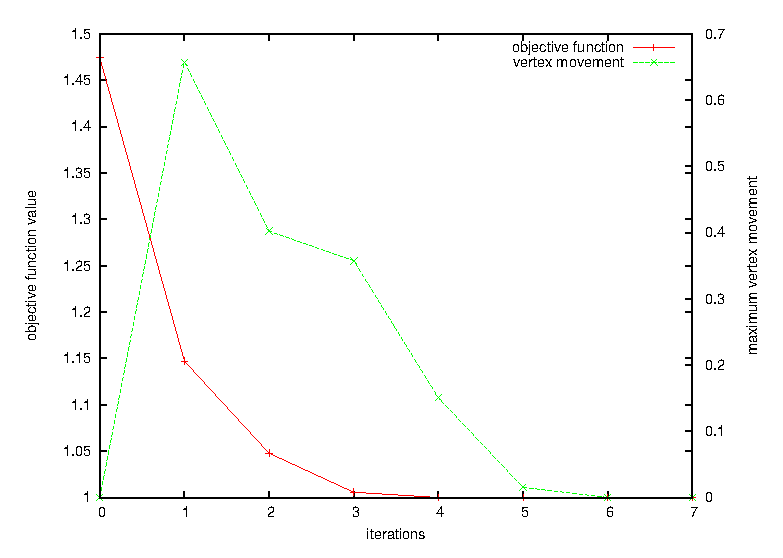
\includegraphics[width=5in]{iterplot}
\caption{\em Convergence Plot \label{fig:iterplot}}
\end{center}
\end{figure}

\section{Viewing Meshes}

VTK files read and written by the {\texttt MeshImpl} class are viewable in a plethora of visualization tools that use the VTK visualization library.  

The {\texttt Mesquite::MeshWriter} namespace contains functions to export mesh in a variety of formats for visualization including:
\begin{itemize}
\item GNU Plot
\item Visualization TookKit (VTK)
\item Encapsulated PostScript (EPS)
\item Scalable Vector Graphics (SVG)
\item StereoLithography (STL)
\end{itemize}
The GNU plot format writes line data that can be used to plot a wireframe of the mesh (the mesh edges).  Both 2D and 3D meshes can be exported in this format.  A mesh can be plotted as a 2D projection with the GNU plot command:
\begin{verbatim}
plot 'filename' with linespoints
\end{verbatim}
or as a rotatable 3D plot with the command:
\begin{verbatim}
splot 'filename' with linespoints
\end{verbatim}
Figure \ref{fig:meshgpt} is the result of plotting the mesh contained in {\texttt testSuite/higher\_order/homogeneousPart.vtk} with GNU plot.

\begin{figure}[htb!]
\begin{center}
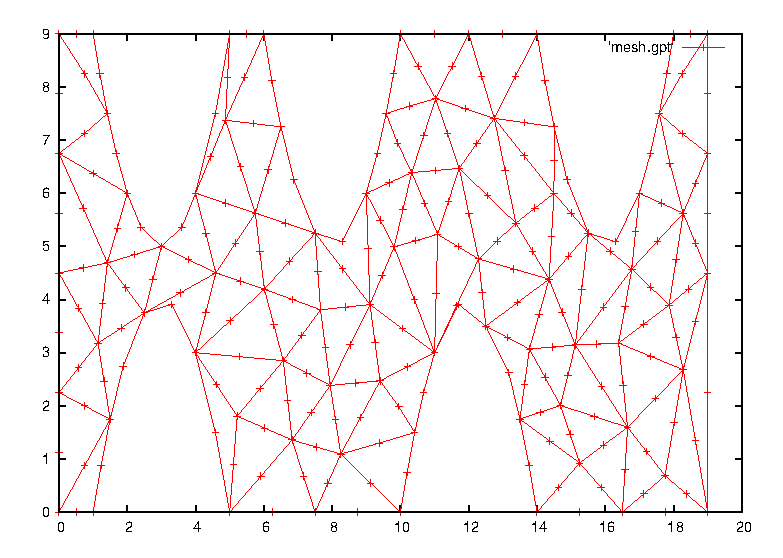
\includegraphics[width=4in]{mesh_gpt}
\caption{\em GNU Plot of 2D Quadratic Triangles \label{fig:meshgpt}}
\end{center}
\end{figure}

As mentioned in the previous section, the VTK file format can be used with a variety of visualization tools.  Figure \ref{fig:meshvtk} shows a simple plot of the same mesh in the Paraview visualization tool.

\begin{figure}[htb!]
\begin{center}
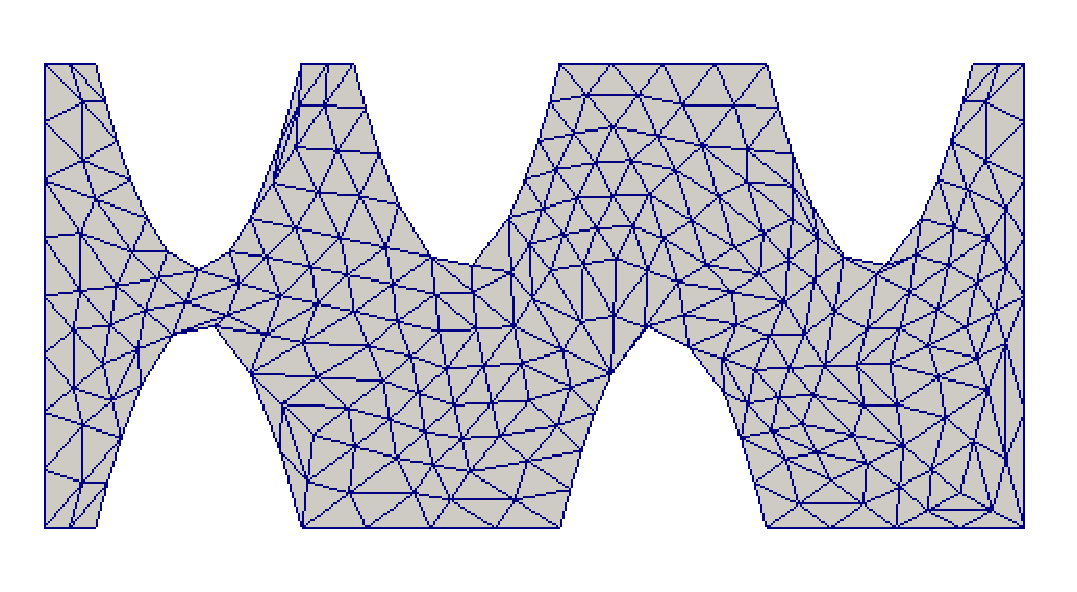
\includegraphics[width=4in]{mesh_vtk}
\caption{\em Paraview plot of 2D Quadratic Triangles \label{fig:meshvtk}}
\end{center}
\end{figure}

Figure \ref{fig:mesh} shows the output of the encapsulated PostScript writer for the mesh.  The EPS writer can write only 2D projections of the mesh.  The caller must specify a projection when calling {\texttt MeshWriter::write\_eps}.  The {\texttt testSuite/higher\_order/homogeneousPart.vtk} file contains quadratic triangle elements.  Compare the mesh edges on the mesh boundary in this plot with the output in Figures \ref{fig:meshgpt} and \ref{fig:meshvtk}.  The EPS writer in Mesquite exports the quadratic edges as curves corresponding to the classic quadratic edge shape function:
\begin{displaymath}
E(u) = \frac{1}{2}u(u-1)V_1 + (1-u^2)V_2 + \frac{1}{2}u(u+1)V_3
\end{displaymath}

\begin{figure}[htb!]
\begin{center}

\includegraphics[width=4in]{mesh}
\caption{\em Encapsulated PostScript of 2D Quadratic Triangles \label{fig:mesh}}
\end{center}
\end{figure}

The STL file format can be used to write only linear triangles.  Higher-order triangular elements will be written as linear triangles.  An error will be returned if the mesh contains other element types.

\section{Exporting Mesh Quality}

The {\texttt QualityAssessor} class has the ability to store mesh quality values and other characteristics as tag data on mesh elements.  This data can be accessed directly by applications or written to a VTK file using the {\texttt MeshImpl} class or the applications native mesh writer (if it is capable of writing tag data.)  The example code below was used to create the VTK file from which the Paraview plot in Figure \ref{fig:meshqual} was generated.

\begin{figure}[htb!]
\begin{center}
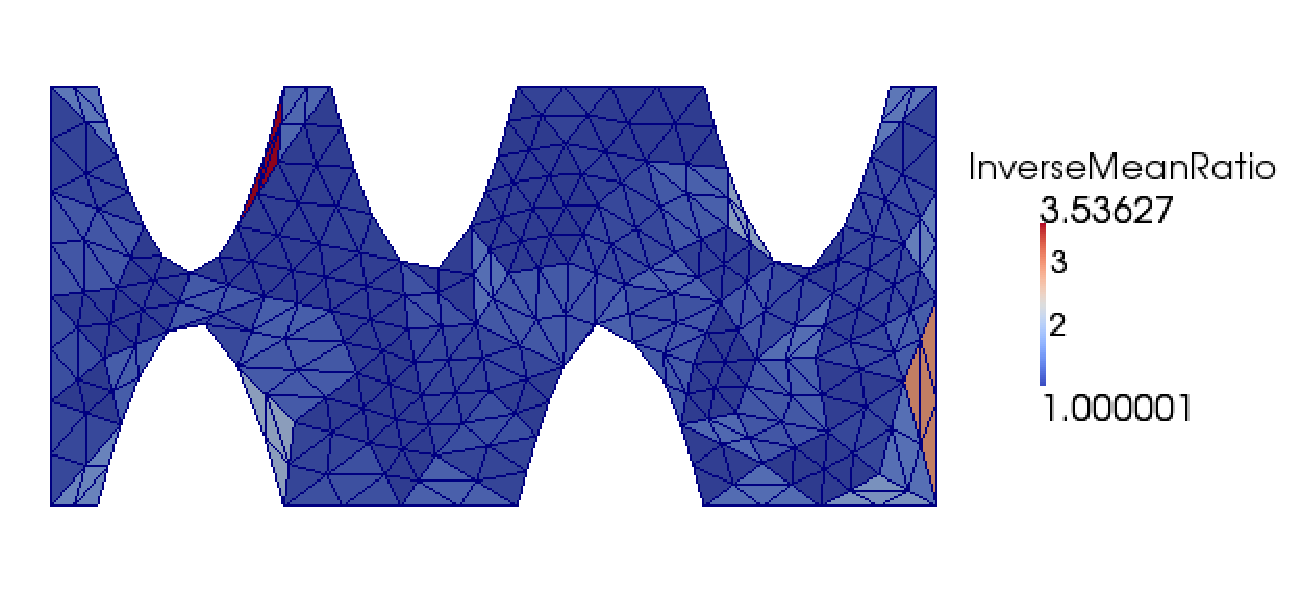
\includegraphics[width=5in]{meshqual}
\caption{\em Paraview Plot Coloring Elements by Quality Metric Value \label{fig:meshqual}}
\end{center}
\end{figure}

\begin{lstlisting}[frame=single]
MsqError err;
MeshImpl mesh;
mesh.read_vtk( "homogeneousPart.vtk", err );

IdealWeightInverseMeanRatio metric;
QualityAssessor qa;
qa.add_quality_assessment(&metric,0,0,0,\<"InverseMeanRatio"\>);

PlanarDomain plane(PlanarDomain::XY);
InstructionQueue queue;
queue.add_quality_assessor( &qa, err );
queue.run_instructions( &mesh, &plane, err );

mesh.write_vtk( "meshqual.vtk", err );
\end{lstlisting}

\begin{figure}[htb!]
\begin{center}
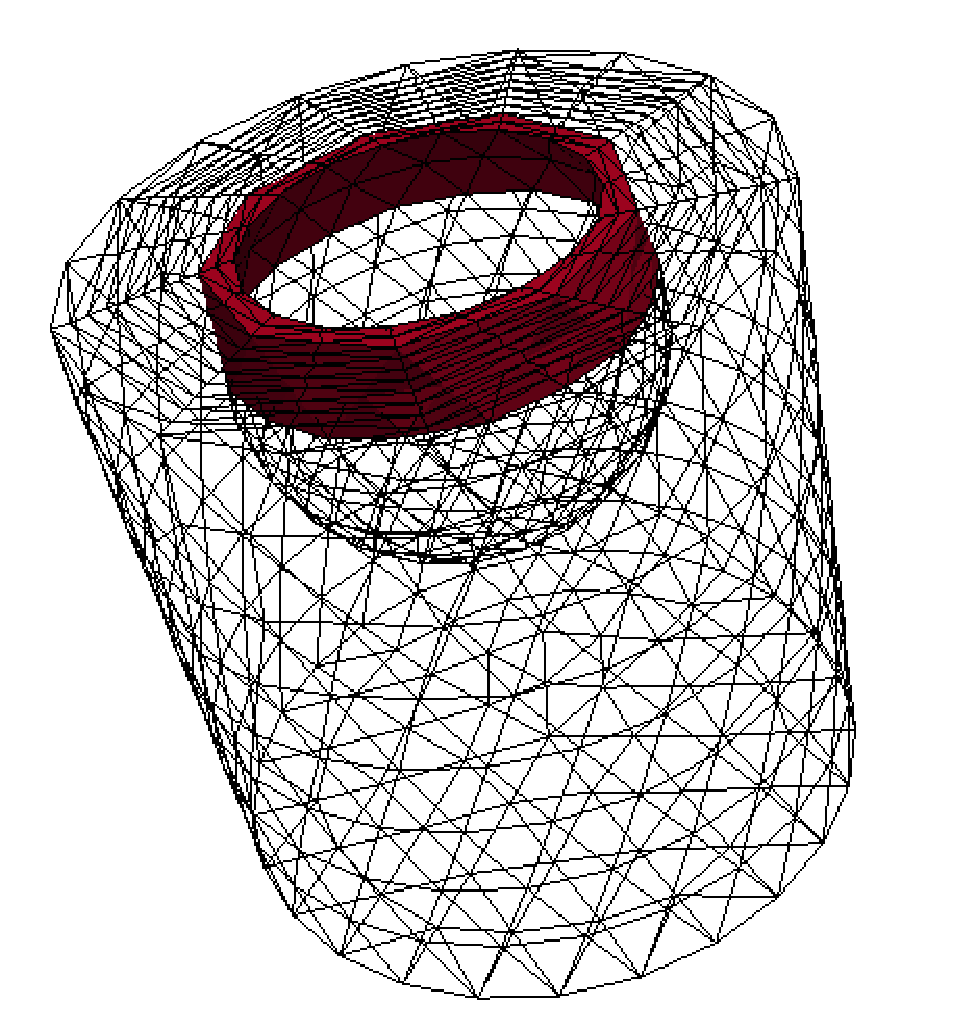
\includegraphics[width=3in]{meshqual3d}
\caption{\em Paraview Plot Showing Inverted Elements \label{fig:meshqual3d}}
\end{center}
\end{figure}

Figure \ref{fig:meshqual3d} is a Paraview plot showing the inverted elements in a quadratic tetrahedral mesh.  The mesh is plotted twice: once as a simple wireframe of the mesh boundary and a second time as solid mesh with a threshold filter on the inverted flag exported by Mesquite.  The listing below shows how the {\texttt QualityAssessor} class can be instructed to flag inverted elements:

\begin{lstlisting}[frame=single]
MsqError err;
MeshImpl mesh;
mesh.read_vtk( "sphereCylinder_1194_inv.vtk", err );

QualityAssessor qa;
\<qa.tag_inverted_elements("Inverted");\>

InstructionQueue queue;
queue.add_quality_assessor( &qa, err );
queue.run_instructions( &mesh, &plane, err );

mesh.write_vtk( "meshqual.vtk", err );
\end{lstlisting}


\section{Mesh Optimization Visualization}

The Mesquite {\texttt TerminationCriterion} class can write the complete mesh after each iteration as either VTK or GNU Plot data suitable for viewing as an animation.  Similar to requesting plot data as described in Section {\ref sec:optplot}, it is important to request this feature from the appropriate termination criterion instance.  If doing a global optimization, the feature should be activated for the {\em inner} termination criterion.  Otherwise the feature should almost always be activated for the {\em outer} termination criterion.  

The command to request an animation of the mesh optimization in the VTK format is:
\begin{lstlisting}
tc.write_mesh_steps( "anim", TerminationCriterion::VTK );
\end{lstlisting}
This will produce a sequence of files named ``anim.1.vtk'', ``anim.2.vtk'', etc.  The files can be opened in visualization tools such as Paraview as a single set and played back as an animation.  If the optimization calculates the gradient of the objective function, that data will also be included in the file as vector data on each mesh vertex.  The components of the vector on each vertex are the partial derivatives of the objective function with respect to each coordinate value of the vertex.  A Paraview ``glyph'' filter can be used to display these vector values during the animation.


The command to request an animation of the mesh optimization in a format suitable for animating in GNU plot is:
\begin{lstlisting}
tc.write_mesh_steps( "anim", TerminationCriterion::GNUPLOT );
\end{lstlisting}
This will produce a sequence of files named ``anim.1'', ``anim.2'', etc.  It will also export a file named ``anim'' that contains the necessary GNU Plot commands to display the animation.



